\documentclass[10pt,aspectratio=43,mathserif]{beamer}
%\usepackage{nju}			 %导入 nju 模板宏包
%\usepackage[UTF8]{ctex}      %导入 ctex 宏包,添加中文支持
\usepackage{xeCJK}
\usepackage{amsmath,amsfonts,amssymb,bm}   %导入数学公式所需宏包
\usepackage{color}			 %字体颜色支持
\usepackage{graphicx,hyperref,url}
\usepackage{listings}
\usepackage{booktabs}
\usepackage{multirow}
\usepackage{float}
\usepackage{mhchem}
\usepackage{animate}
\usepackage[isbn=false,doi=false,uniquename=init]{biblatex}
\addbibresource{icc_pre_1108.bib}
\AtEveryCitekey{\clearfield{title}}
\AtEveryBibitem{\clearfield{title}}
\usepackage{textcomp}

%\beamertemplateballitem		%设置 Beamer 主题
%\catcode`\。=\active        %或者=13
%\newcommand{。}{.}         %将正文中的“。”号转换为“.”。

%\AtBeginSection[]
%{
%  \begin{frame}
%    \frametitle{Contents}
%    \tableofcontents[currentsection]
%  \end{frame}
%}



\title{Theoretical Investigation on $ S_N 2 $ with/without Solvation}	        %首页信息设置

\author[]{            %个人信息设置
    Shirong Wang\\[0.3cm]
    %15XXXXXXXX\\[0.3cm]
    Kuang Yaming Honors School}

\date{\today}



\begin{document}

\begin{frame}
\titlepage
\end{frame}

\begin{frame}
\frametitle{Contents}
\tableofcontents
\end{frame}

\section{Reaction I}
\begin{frame}
\frametitle{Oxidative addition of $ \ce{Pt(PMe_3)_2} $}
\begin{equation}\label{key}
\ce{Pt(PMe_3)_2 + H_2 -> Pt(PMe_3)_2H_2}
\end{equation}

\end{frame}

\begin{frame}
\textbf{Question:} \textsl{cis} or \textsl{trans} product?\\

\begin{figure}[H]
	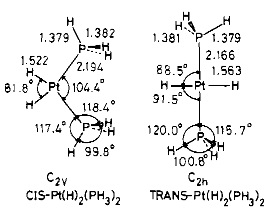
\includegraphics[width=0.45\linewidth]{Pt1.jpg}
\end{figure}
Only \textsl{cis} product is symmetry allowed. (\textsl{cis} product can be converted into \textsl{trans}, although)\\

\fullcite{Kitaura1981}
%\nocite{Kitaura1981}
%\printbibliography
\end{frame}

\begin{frame}
\frametitle{TS}
\begin{figure}
	\animategraphics[width=0.45\linewidth,loop,autoplay]{30}{../Pt/pbe0/vib/Pt_tsb000}{00}{47}
	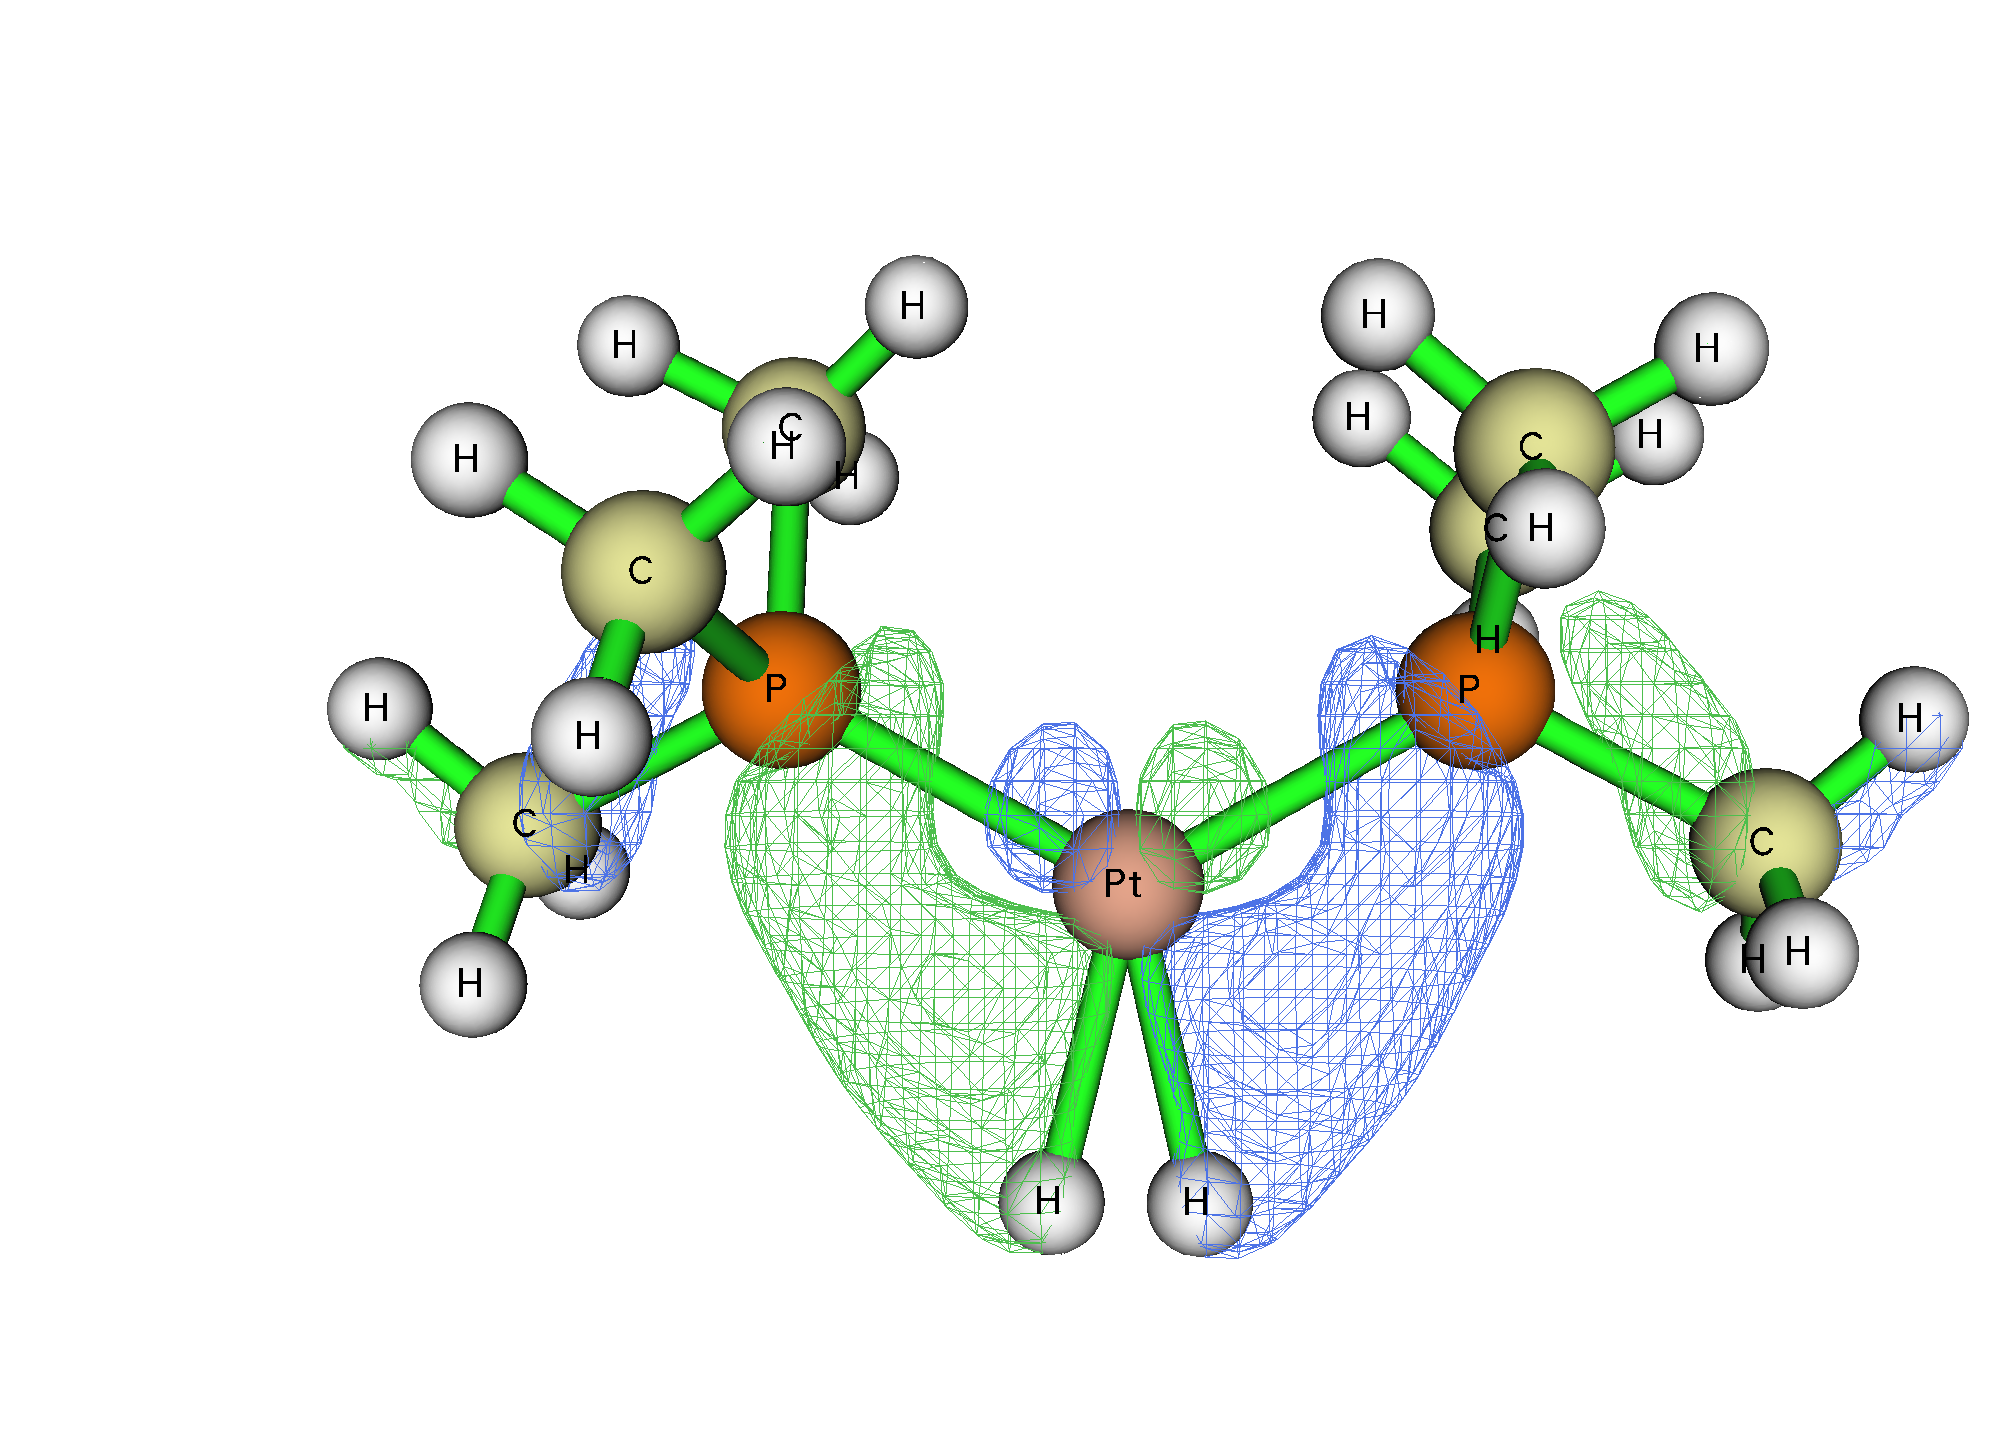
\includegraphics[width=0.45\linewidth]{Pt_tsb_orb.png}
\end{figure}
Calculated at PBE0/def2-TZVP.
\end{frame}

\begin{frame}
\begin{figure}
	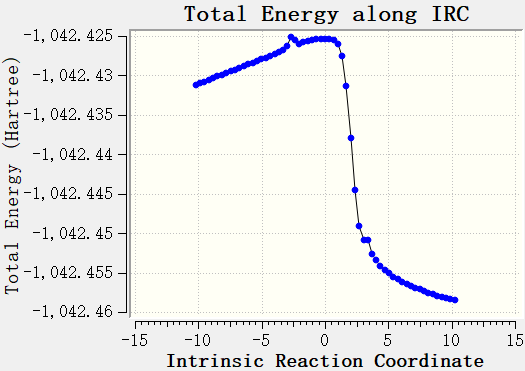
\includegraphics[width=0.45\linewidth]{../Pt/Pt_ircb2.png}
\end{figure}
\begin{figure}
	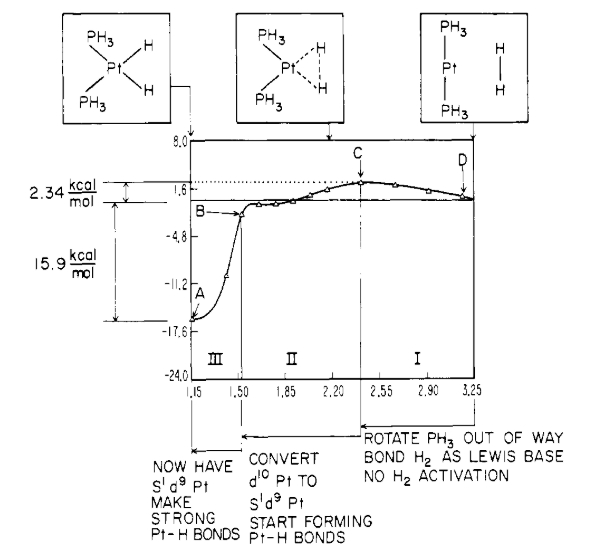
\includegraphics[width=0.45\linewidth]{god1.jpg}
	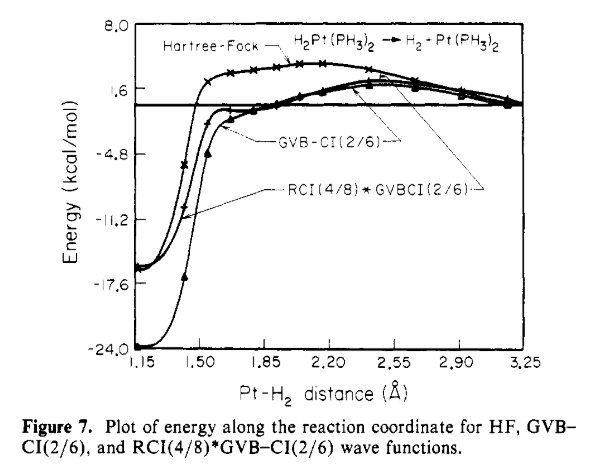
\includegraphics[width=0.45\linewidth]{god2.jpg}
\end{figure}
\fullcite{Goddard1984}
\end{frame}

\begin{frame}
\begin{figure}
	%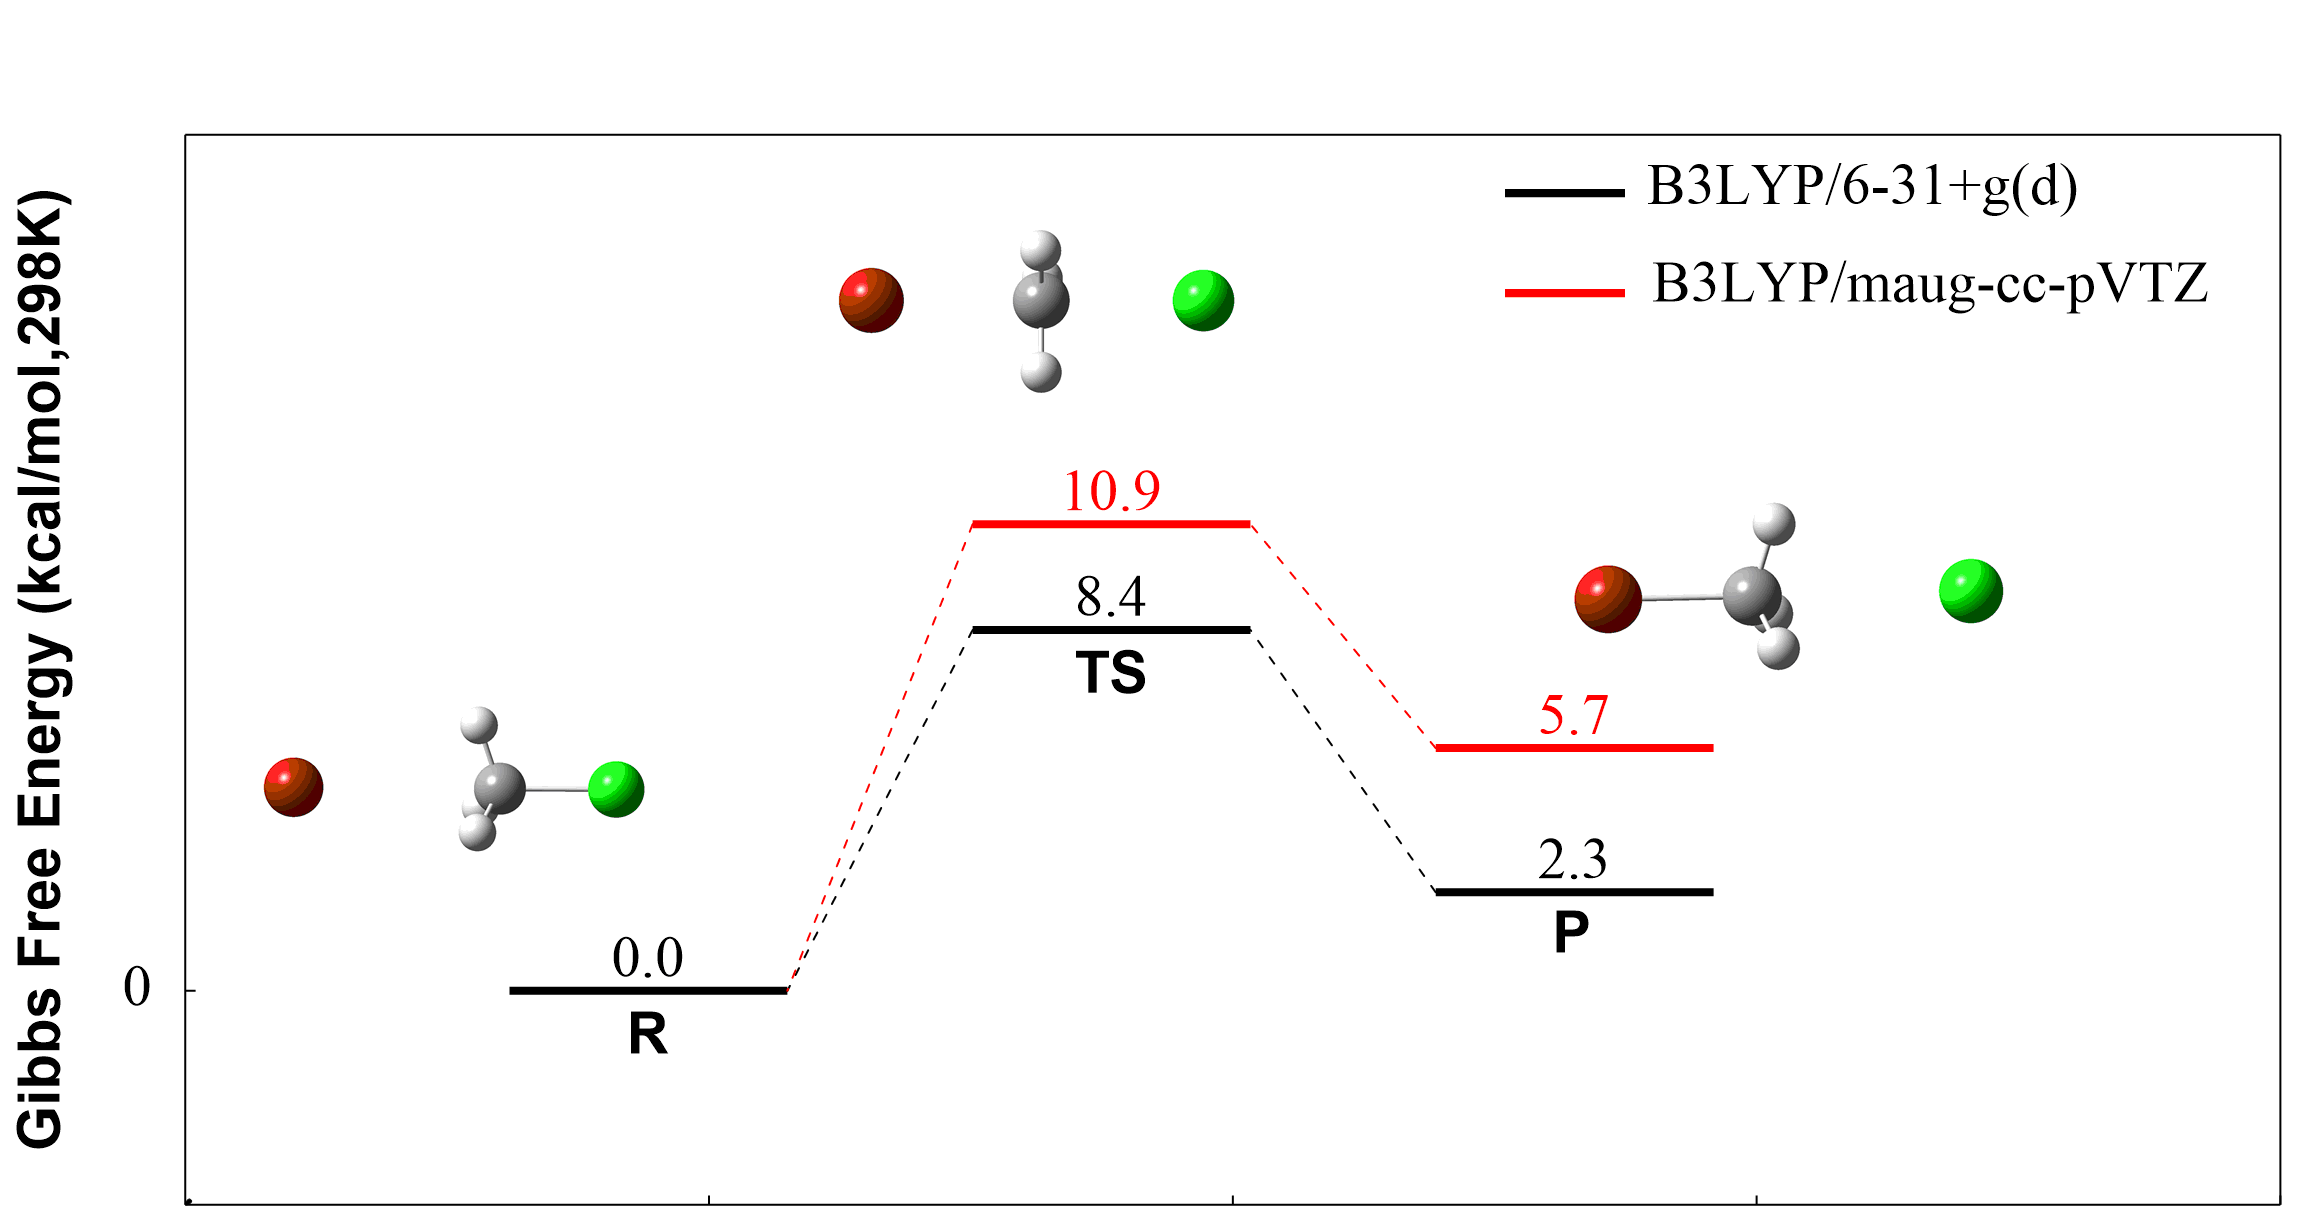
\includegraphics[width=\linewidth]{../sample/sn2c.png}
\end{figure}
\begin{table}[H]
	\centering
	\begin{tabular}{ccccc}
		\hline
		& $ R_{\ce{PtH}} $(TS) & $ R_{\ce{PtH}} $(P) & $ A_{\ce{HPtH}} $(TS) & $ A_{\ce{HPtH}} $(P)\\ \hline
		M06-2X/SDD/6-31g* & 1.860 &  & 26.22 &  \\
		%HF & 1.81 & 1.55 &  &  \\
		\hline
	\end{tabular}
    \caption{Bond length (\AA) and bond angle (\textdegree) in configurations above}
\end{table}
\begin{table}[H]
	\centering
	\begin{tabular}{cccc}
		\hline
		& R & TS & P \\ \hline
		$ E_{elec} $(B2PLYPD3/def2-TZVP) &  &  &    \\
		$ \Delta G_{freq} $(M06-2X/SDD/6-31g*) &  &  &    \\
		$ \Delta G_{sol} $(M06-2X/SDD/6-31g*) & & & \\
		\hline
	\end{tabular}
	\caption{Energies}
\end{table}
\end{frame}


\section{Reaction III}
\begin{frame}


%\printbibliography
\end{frame}
%\bibliography{icc_pre_1108}
%\bibliographystyle{plain}


\end{document}